\section*{Problem 3.9}
Numerically solve the Hamiltonian Eq. 3.92 for a finite number of particles, and discuss the wave function, density matrix, and relative particle fluctuations in three regimes (i) $U>0$ and $ U \ll J$; (ii)$U>0$ and $U \gg J$; and (iii)$U<0$ and $\left\lvert U\right\rvert \gg J$. In regime (iii), also discuss the excitation gap between the first excited state and the ground state as a function of total prticle number N.
\paragraph*{Solution:}
% wave function
For N particles, using the Fork states $\left\{ \ket{n, N-n}\right\}$ as the basis, the wave function in three regimes are plotted as Fig. \ref{3.9 fig wf}

\begin{figure}[h]
    \centering
    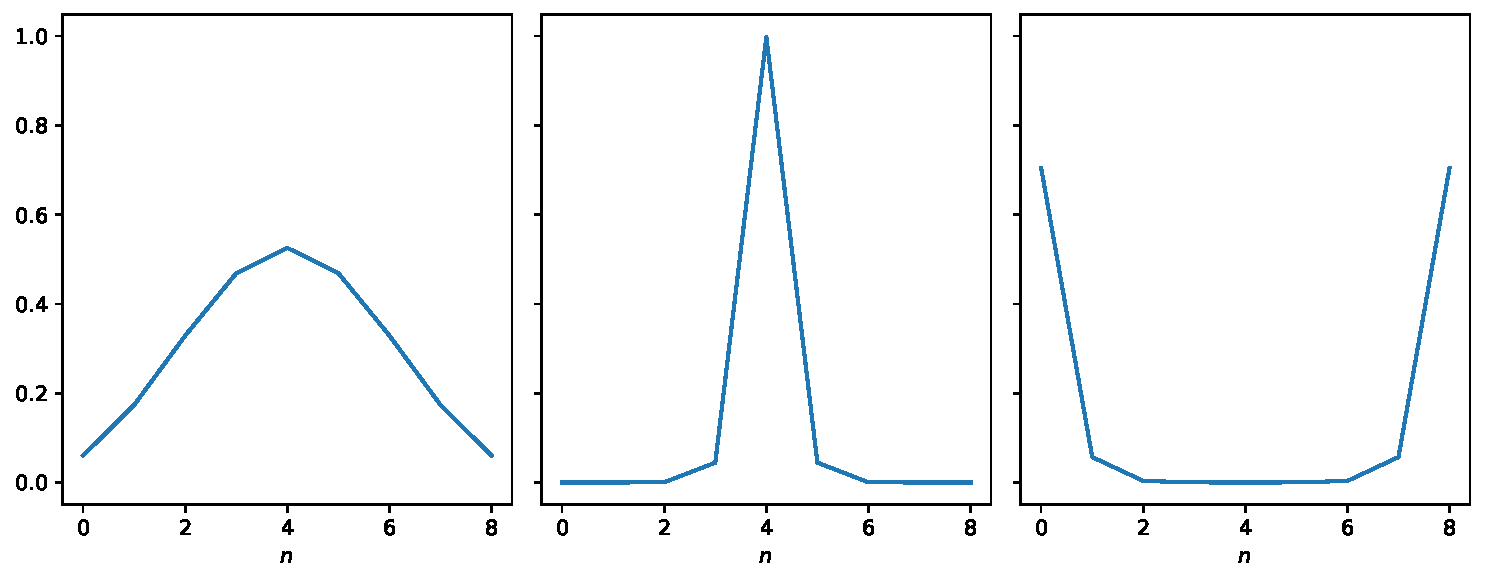
\includegraphics[width=.8\textwidth]{wf.pdf}
    \caption{Wave function}
    \label{3.9 fig wf}
\end{figure}

% density matrix
The density matrix are
\begin{minted}{text}
    [[0.004 0.01  0.02  0.028 0.032 0.028 0.02  0.01  0.004]
    [0.01  0.03  0.057 0.081 0.091 0.081 0.057 0.03  0.01 ]
    [0.02  0.057 0.108 0.154 0.173 0.154 0.108 0.057 0.02 ]
    [0.028 0.081 0.154 0.22  0.246 0.22  0.154 0.081 0.028]
    [0.032 0.091 0.173 0.246 0.276 0.246 0.173 0.091 0.032]
    [0.028 0.081 0.154 0.22  0.246 0.22  0.154 0.081 0.028]
    [0.02  0.057 0.108 0.154 0.173 0.154 0.108 0.057 0.02 ]
    [0.01  0.03  0.057 0.081 0.091 0.081 0.057 0.03  0.01 ]
    [0.004 0.01  0.02  0.028 0.032 0.028 0.02  0.01  0.004]]
   [[0.    0.    0.    0.    0.    0.    0.    0.    0.   ]
    [0.    0.    0.    0.    0.    0.    0.    0.    0.   ]
    [0.    0.    0.    0.    0.    0.    0.    0.    0.   ]
    [0.    0.    0.    0.002 0.044 0.002 0.    0.    0.   ]
    [0.    0.    0.    0.044 0.996 0.044 0.    0.    0.   ]
    [0.    0.    0.    0.002 0.044 0.002 0.    0.    0.   ]
    [0.    0.    0.    0.    0.    0.    0.    0.    0.   ]
    [0.    0.    0.    0.    0.    0.    0.    0.    0.   ]
    [0.    0.    0.    0.    0.    0.    0.    0.    0.   ]]
   [[0.497 0.04  0.003 0.    0.    0.    0.003 0.04  0.497]
    [0.04  0.003 0.    0.    0.    0.    0.    0.003 0.04 ]
    [0.003 0.    0.    0.    0.    0.    0.    0.    0.003]
    [0.    0.    0.    0.    0.    0.    0.    0.    0.   ]
    [0.    0.    0.    0.    0.    0.    0.    0.    0.   ]
    [0.    0.    0.    0.    0.    0.    0.    0.    0.   ]
    [0.003 0.    0.    0.    0.    0.    0.    0.    0.003]
    [0.04  0.003 0.    0.    0.    0.    0.    0.003 0.04 ]
    [0.497 0.04  0.003 0.    0.    0.    0.003 0.04  0.497]]
\end{minted}

% relative particle fluctuations
The relative particle fluctuations in three regimes are 
\begin{minted}{text}
    [7.863081011461077, 0.015831682417565402, 63.817067740969534]
\end{minted}
in first regime, $\braket{(\Delta \hat{N})^2} \approx  N$, in second regime, $\braket{(\Delta \hat{N})^2} \approx 0$, and in third regime, $\braket{(\Delta \hat{N})^2} \approx N^2$, which is consistent with the theoretically results.

% excitation gap
The excitation gap as a function of total particle number N is plotted as

\begin{figure}[h]
    \centering
    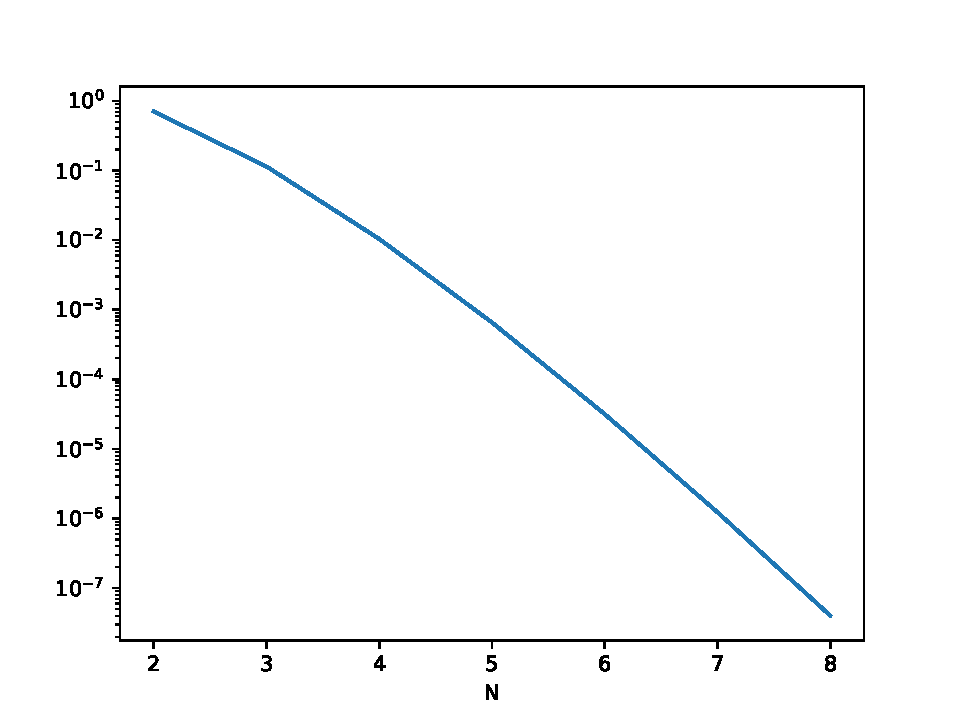
\includegraphics[width=.8\textwidth]{gap.pdf}
    \caption{Excitation gap}
    \label{3.9 fig gap}
\end{figure}

So as the number N increases, the excitation gap is close to zero, which means the ground state and the first excited state degenerate. While the ground state is symmetric and the first excited state is antisymmetric, this implies spontaneous symmetry breaking.